		\begin{enumerate}
			\item The \emph{projection} of $\vec v$ onto $X$ is the closest point in $X$ to $\vec v$.
			\item \begin{enumerate}
					\item $\phantom{x}$

\begin{center}
	\begin{tikzpicture}[scale=.8, >=latex]
    \begin{axis}[scale=1,
		    axis equal image,
		    %axis line style={draw=none},
		    axis lines=middle,
		    tick style={draw=none},
		    yticklabels={,,},
		    xticklabels={,,},
		 xmin=-.5,
		 xmax=1.5,
		 ymin=-.5,
		 ymax=1.5,
		 major grid style={dotted, gray},
                 xtick={-10,-9,...,10},
                 ytick={-10,-9,...,10},
                 grid=both,
		 anchor=origin]

	  \draw[green!50!black, very thick]
	    (0,0)-- (0,1)--
	    (1,1) node[above right, black] {$R$}-- (1,0) -- cycle
	    ;
    \end{axis}
\end{tikzpicture}
	\begin{tikzpicture}[scale=.8, >=latex]
    \begin{axis}[scale=1,
		    axis equal image,
		    %axis line style={draw=none},
		    axis lines=middle,
		    tick style={draw=none},
		    yticklabels={,,},
		    xticklabels={,,},
		 xmin=-.5,
		 xmax=1.5,
		 ymin=-.5,
		 ymax=1.5,
		 major grid style={dotted, gray},
                 xtick={-10,-9,...,10},
                 ytick={-10,-9,...,10},
                 grid=both,
		 anchor=origin]

	  \fill[fill=blue]
	    (0,0) circle[radius=2pt] (0,1) circle[radius=2pt]
	    (1,1) circle[radius=2pt] node[above right] {$C$} (1,0) circle[radius=2pt]
	    ;
    \end{axis}
\end{tikzpicture}
	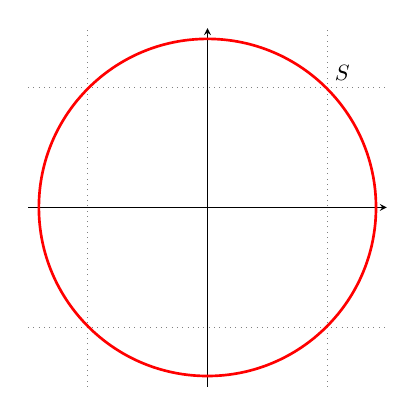
\begin{tikzpicture}[scale=.8, >=latex]
    \begin{axis}[scale=1,
		    axis equal image,
		    %axis line style={draw=none},
		    axis lines=middle,
		    tick style={draw=none},
		    yticklabels={,,},
		    xticklabels={,,},
		 xmin=-1.5,
		 xmax=1.5,
		 ymin=-1.5,
		 ymax=1.5,
		 major grid style={dotted, gray},
                 xtick={-10,-9,...,10},
                 ytick={-10,-9,...,10},
                 grid=both,
		 anchor=origin]

	  \draw[red, very thick]
	    (0,0) circle[radius=1.41]
	    ;
	   \path (1,1) node[above right] {$S$};
    \end{axis}
\end{tikzpicture}
\end{center}
					\item $\phantom{x}$

\begin{center}
	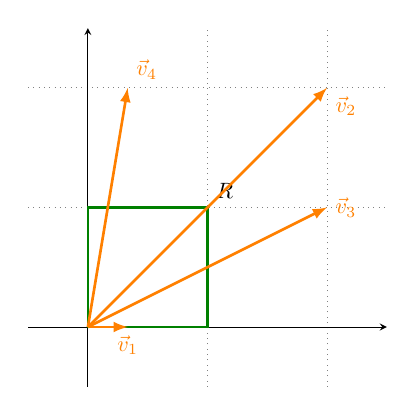
\begin{tikzpicture}[scale=.8, >=latex]
    \begin{axis}[scale=1,
		    axis equal image,
		    %axis line style={draw=none},
		    axis lines=middle,
		    tick style={draw=none},
		    yticklabels={,,},
		    xticklabels={,,},
		 xmin=-.5,
		 xmax=2.5,
		 ymin=-.5,
		 ymax=2.5,
		 major grid style={dotted, gray},
                 xtick={-10,-9,...,10},
                 ytick={-10,-9,...,10},
                 grid=both,
		 anchor=origin]

	  \draw[green!50!black, very thick]
	    (0,0)-- (0,1)--
	    (1,1) node[above right, black] {$R$}-- (1,0) -- cycle
	    ;
	    \draw[orange, ->, very thick] (0,0) -- (.333,0) node[below] {$\vec v_1$};
	    \draw[orange, ->, very thick] (0,0) -- (2,2) node[below right] {$\vec v_2$};
	    \draw[orange, ->, very thick] (0,0) -- (2,1) node[right] {$\vec v_3$};
	    \draw[orange, ->, very thick] (0,0) -- (.333,2) node[above right] {$\vec v_4$};
    \end{axis}
\end{tikzpicture}
	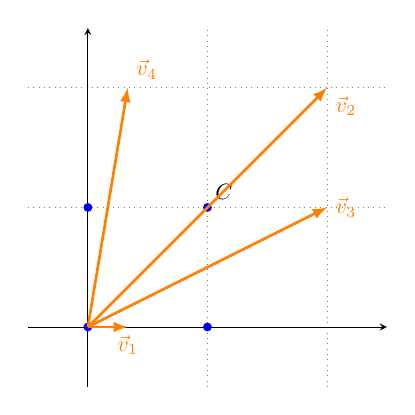
\begin{tikzpicture}[scale=.8, >=latex]
    \begin{axis}[scale=1,
		    axis equal image,
		    %axis line style={draw=none},
		    axis lines=middle,
		    tick style={draw=none},
		    yticklabels={,,},
		    xticklabels={,,},
		 xmin=-.5,
		 xmax=2.5,
		 ymin=-.5,
		 ymax=2.5,
		 major grid style={dotted, gray},
                 xtick={-10,-9,...,10},
                 ytick={-10,-9,...,10},
                 grid=both,
		 anchor=origin]

	  \fill[fill=blue]
	    (0,0) circle[radius=2pt] (0,1) circle[radius=2pt]
	    (1,1) circle[radius=2pt] node[above right] {$C$} (1,0) circle[radius=2pt]
	    ;
	    \draw[orange, ->, very thick] (0,0) -- (.333,0) node[below] {$\vec v_1$};
	    \draw[orange, ->, very thick] (0,0) -- (2,2) node[below right] {$\vec v_2$};
	    \draw[orange, ->, very thick] (0,0) -- (2,1) node[right] {$\vec v_3$};
	    \draw[orange, ->, very thick] (0,0) -- (.333,2) node[above right] {$\vec v_4$};
    \end{axis}
\end{tikzpicture}
	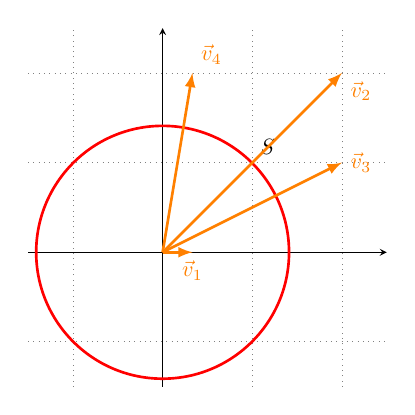
\begin{tikzpicture}[scale=.8, >=latex]
    \begin{axis}[scale=1,
		    axis equal image,
		    %axis line style={draw=none},
		    axis lines=middle,
		    tick style={draw=none},
		    yticklabels={,,},
		    xticklabels={,,},
		 xmin=-1.5,
		 xmax=2.5,
		 ymin=-1.5,
		 ymax=2.5,
		 major grid style={dotted, gray},
                 xtick={-10,-9,...,10},
                 ytick={-10,-9,...,10},
                 grid=both,
		 anchor=origin]

	  \draw[red, very thick]
	    (0,0) circle[radius=1.41]
	    ;
	   \path (1,1) node[above right] {$S$};
	    \draw[orange, ->, very thick] (0,0) -- (.333,0) node[below] {$\vec v_1$};
	    \draw[orange, ->, very thick] (0,0) -- (2,2) node[below right] {$\vec v_2$};
	    \draw[orange, ->, very thick] (0,0) -- (2,1) node[right] {$\vec v_3$};
	    \draw[orange, ->, very thick] (0,0) -- (.333,2) node[above right] {$\vec v_4$};
    \end{axis}
\end{tikzpicture}
\end{center}

	\item
		\[
			\Proj_R\vec v_1=\vec v_1\qquad
			\Proj_R\vec v_2=\mat{1\\1}\qquad
			\Proj_R\vec v_3=\mat{1\\1}\qquad
			\Proj_R\vec v_4=\mat{1/3\\1}
		\]
		\[
			\Proj_C\vec v_1=\mat{0\\0}\qquad
			\Proj_C\vec v_2=\mat{1\\1}\qquad
			\Proj_C\vec v_3=\mat{1\\1}\qquad
			\Proj_C\vec v_4=\mat{0\\1}
		\]
		\[
			\Proj_S\vec v_1=\mat{\sqrt{2}\\0}\qquad
			\Proj_S\vec v_2=\mat{1\\1}\qquad
			\Proj_S\vec v_3=\frac{\sqrt{2}\vec v_3}{\|\vec v_3\|}\qquad
			\Proj_S\vec v_4=\frac{\sqrt{2}\vec v_4}{\|\vec v_4\|}
		\]

\end{enumerate}

	\item \begin{enumerate}
			\item $f(t) = \sqrt{(t-2)^2+(2t-2)^2} = \sqrt{5t^2-12t+8}$.
			\item $\Proj_\ell \vec r$ must be the multiple of $\vec d$ that is
				closest to $\vec r$. Notice that $f(t)$ is minimized when
				$5t^2-12t+8$ is minimized which happens when $t=6/5$. Therefore
				\[
					\Proj_\ell \vec r = \tfrac{6}{5}\mat{1\\2}.
				\]
			\item $90^\circ$.
			\item They are the same thing! To find the closest point on a line
				to a point, you draw a perpendicular to the line passing through the point.
				The intersection with the line is the closest point and is therefore the projection.
				However, the line in this case is given by
				all multiples of $\vec d$, so geometrically,
				$\Comp_{\vec d}\vec r$ is defined in the exact same way as $\Proj_\ell \vec r$ (in this case).
	\end{enumerate}
		\item  \begin{enumerate}
				\item $\mat{x\\y}\mapsto \mat{x\\0}$.
			\item Let $\vec d=\mat{2\\1}$ and $\vec x=\mat{x\\y}$.
				Then $\vec x\mapsto \Comp_{\vec d}\vec x = \frac{2x+y}{5}\mat{2\\1}$.
			\item Let $\vec s=\mat{-1\\2}$ be the direction of the sunlight and let $\vec x$ be as before.
				We are looking for when $\vec x+t\vec s$ has a zero $y$-coordinate, which happens when
				$t=-y/2$. Therefore
				\[
					\mat{x\\y}\mapsto \mat{x\\y}+\tfrac{-y}{2}\mat{-1\\2} = \mat{x+y/2\\0}.
				\]
		\end{enumerate}

		\end{enumerate}
	
